\hypertarget{muxe9thodologie}{%
\subsection{Méthodologie}\label{muxe9thodologie}}

Notre idée centrale est de porter l'analyse sur la différence entre les
deux journaux et leur évolution dans le temps. La méthodologie détaillée
ici est donc appliquée sur les deux journaux séparément et elle est
organisé de manière suivante:

\begin{figure}
\centering
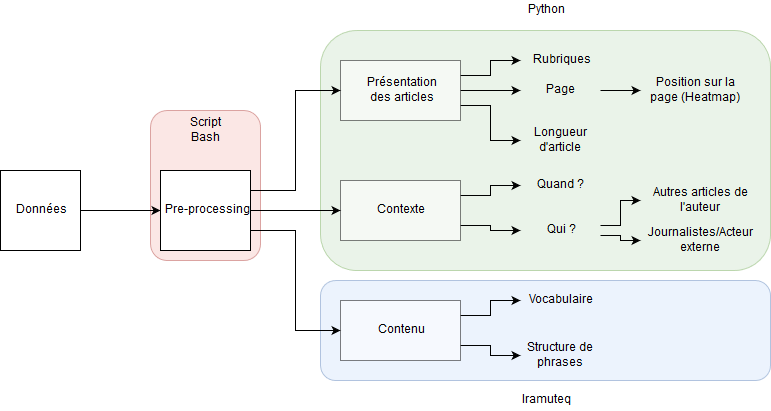
\includegraphics[width=0.7\textwidth,height=\textheight]{methods.png}
\caption{Organisation et outils de l'analyse.}
\end{figure}

\hypertarget{pre-processing}{%
\subsubsection{Pre-processing}\label{pre-processing}}

Pour l'explorer de manière plus rapide, nous devons réduire le corpus de
base qui se constitue des articles de la \emph{Gazette de Lausanne}
(\emph{GDL}) et du \emph{Journal de Genève} (\emph{JDG}) sortis entre
1900 et 1999.

Nous créons trois corpus. Le plus grand est constitué de tous les
articles, décomprimés (du format \texttt{bzip2}) et sans méta-données
concernant la position des mots sur la page. Nous nous servons de ce
corpus-là pour des questions qui regardent l'entièreté des journaux,
comme la longueur en page du journal à une certaine date.

Le deuxième corpus se limite aux articles de caractère financier et est
extrait du premier corpus par la recherche des mots clés suivants:

\begin{itemize}
\tightlist
\item
  secret bancaire
\item
  place financière
\item
  banques suisses
\item
  forfait fiscal
\item
  paradis fiscal
\item
  affaire Chiasso
\item
  argent sale
\item
  blanchiment
\end{itemize}

Nous utilisons ce corpus de \textasciitilde{}35'000 articles pour nous
comparer avec notre troisième corpus, sélectionné par le seul mot clé
``secret bancaire'', contentant environ 1700 articles. De cette façon,
nous pouvons déterminer si une certaine tendance de ce corpus est
vraiment signifiante, ou si elle apparaît dans tout le corpus financier.

\hypertarget{statistiques-de-base}{%
\subsubsection{Statistiques de base}\label{statistiques-de-base}}

Nous commençons en calculant certaines statistiques de base, telles que
le numéro de page, la longueur et la date d'un article. Nous
reproduisons donc le N-Gram dans le temps, pour les articles contenant
``secret bancaire'' par année.

\begin{figure}
\centering
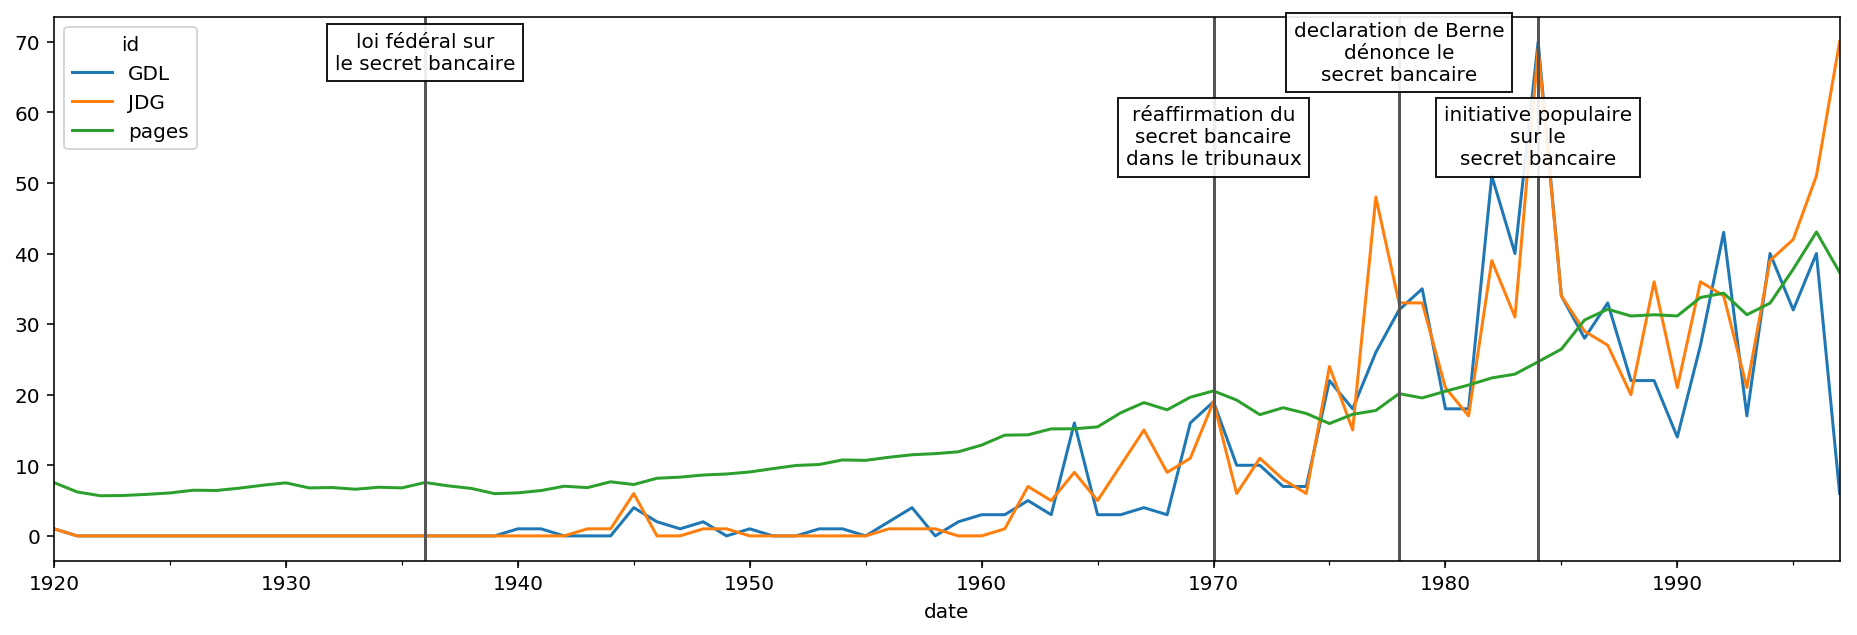
\includegraphics{ngram_ts.png}
\caption{Apparitions du terme ``secret bancaire'' dans les deux journaux
au cours du temps}
\end{figure}

Ensuite, nous comparons la longueur d'un article sur le secret bancaire
aux articles génériques du corpus financier. Nous pouvons constater en
regardant l'histogramme suivant que les articles sur le secret bancaire,
dans les deux journaux, sont en général un peu plus longs.

\begin{figure}
\centering
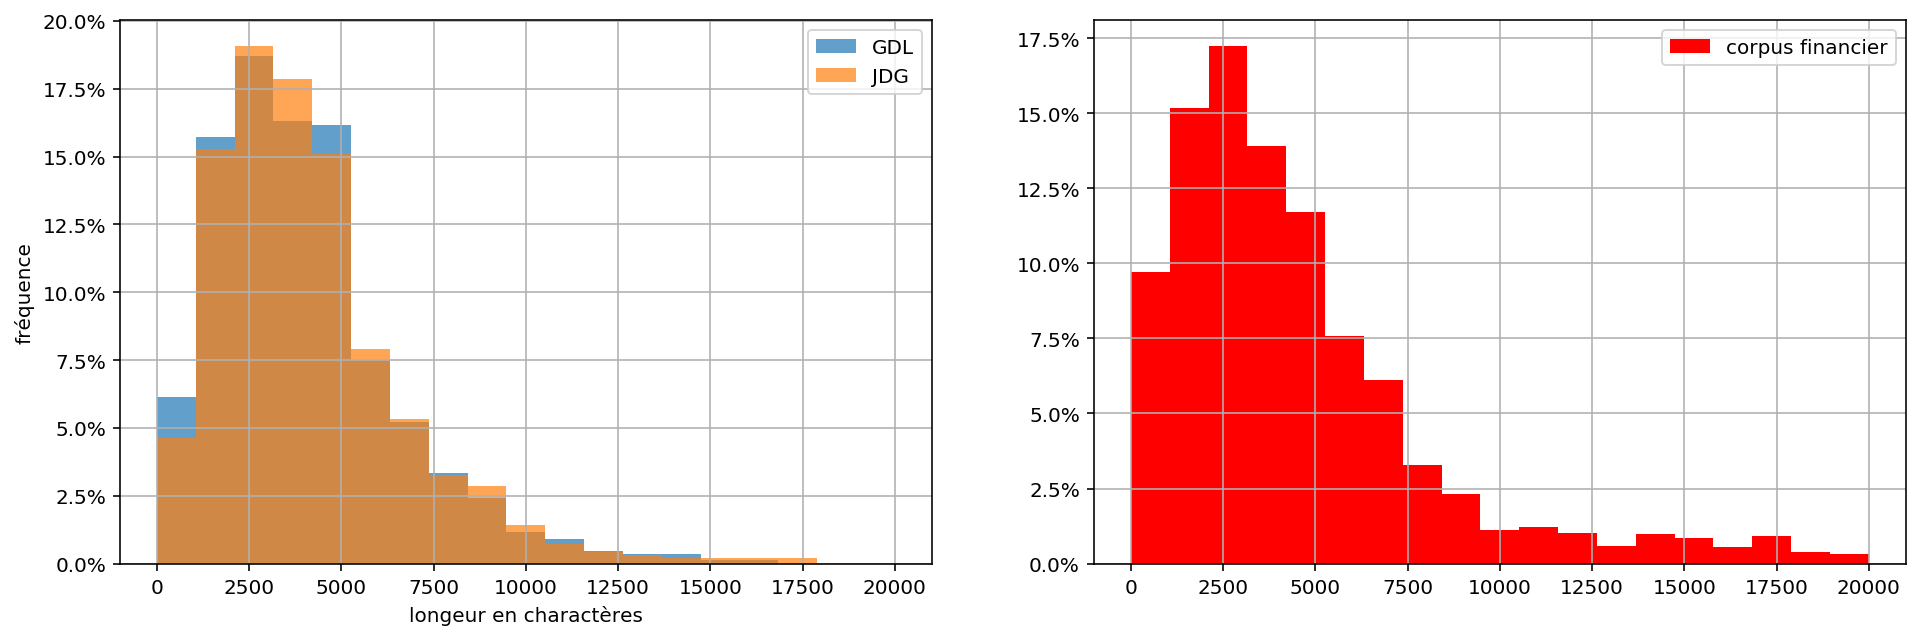
\includegraphics[width=0.6\textwidth,height=\textheight]{article_lengths.png}
\caption{Distribution de la longueur des articles}
\end{figure}

Nous examinons aussi, à l'aide d'un histogramme de la page de l'article,
la distribution de la position des articles sur le secret bancaire. Pour
mieux interpréter les résultats de cette analyse, nous trouvons la
longueur du journal pour chaque date et calculons ainsi la position
relative de l'article dans le journal. Nous cherchons enfin à voir si
des rubriques spécialisées traitent le sujet, en examinant des nuages de
points corrélants la date et la page des articles en question. Des ligne
horizontales isolées constituerait un indice d'une rubrique permanente.

\begin{figure}
\centering
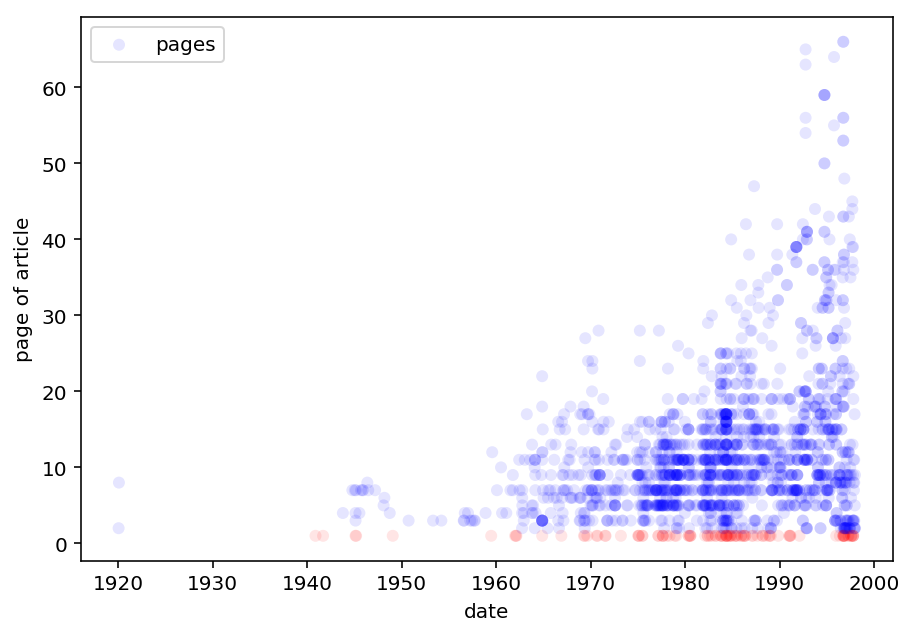
\includegraphics[width=0.5\textwidth,height=\textheight]{scatter.png}
\caption{Nuage de points de la page des articles dans le temps}
\end{figure}

En comparant le nombre d'article en première page, nous constatons que
la fréquence d'une première page pour un article sur le secret bancaire
est de 5\% dans la \emph{GDL} et 6\% dans le \emph{JDG}. Alors que la
fréquence d'une première page pour un article générique financier est de
2\% pour la \emph{GDL} et 3\% pour la \emph{JDG}.

\hypertarget{analyse-des-auteurs}{%
\subsubsection{Analyse des auteurs}\label{analyse-des-auteurs}}

La méta-donnée la plus importante après la date qui est traitée en haut
est l'auteur d'un article. Nous analysons deux catégories d'auteurs.

\hypertarget{agences-de-presse}{%
\paragraph{Agences de presse}\label{agences-de-presse}}

Beaucoup d'articles de journal proviennent d'agences de presse externes
à la rédaction. Nous classifions les articles des agences suivantes:

\begin{itemize}
\tightlist
\item
  ATS: Agence télégraphique suisse
\item
  AFP: Agence France-Presse
\item
  Reuters
\item
  AP: Associated press
\end{itemize}

Ainsi nous trouvons que pour les articles du secret bancaire le taux
d'articles issus d'agences et 10\% plus haut que dans le corpus
financier.

\newpage

\hypertarget{journalistes}{%
\paragraph{Journalistes}\label{journalistes}}

Même si l'auteur n'est pas toujours indiqué -- surtout dans la première
moitié du siècle -- nous arrivons à extraire des données sur les
journalistes. Au moyen d'une liste de noms d'auteurs\footnote{Cette
  liste était obtenue de la page
  \href{https://fr.wikipedia.org/wiki/Journal_de_Gen\%C3\%A8ve}{Wikipédia
  du \emph{Journal de Genève}}.} et des initiales à la fin de l'article,
nous pouvons attribuer des auteurs à plus que 2600 articles.

\begin{figure}
\centering
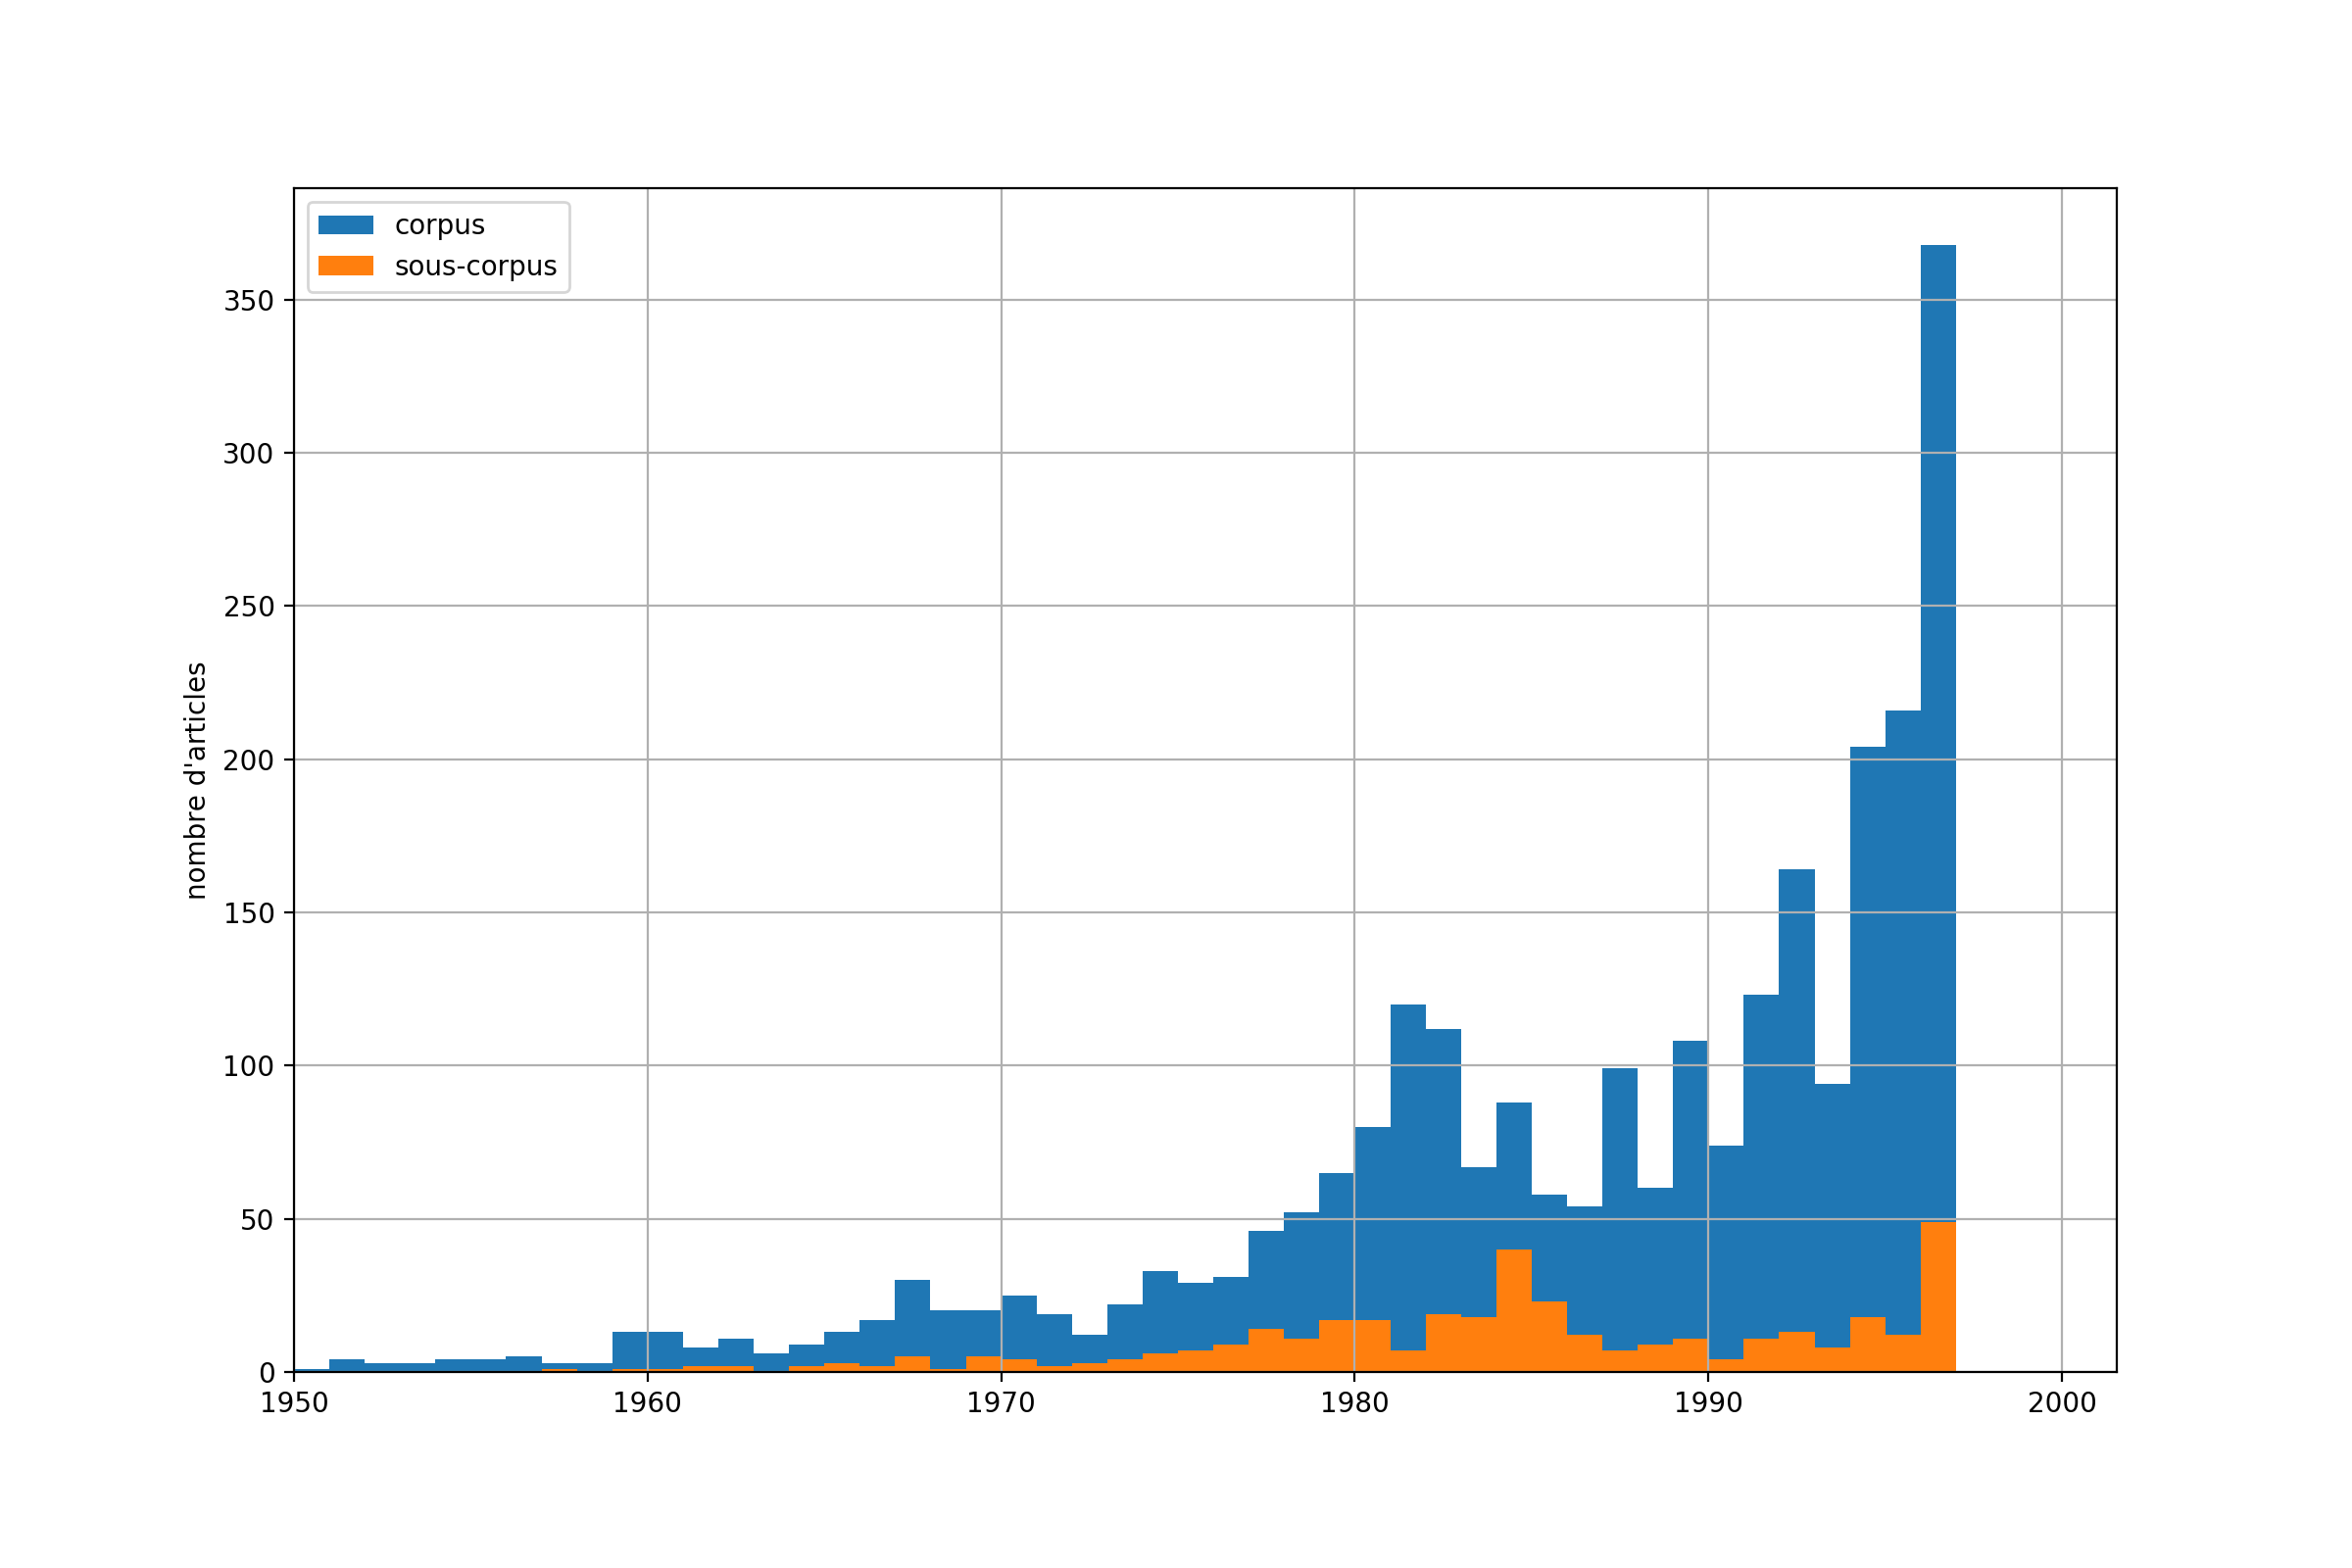
\includegraphics[width=0.6\textwidth,height=\textheight]{author_attributed.png}
\caption{Articles avec auteur attribué}
\end{figure}

Cette attribution nous permet de poser les questions suivantes: Est-ce
qu'un journaliste est actif dans le deux journaux en même temps? Est-ce
qu'il écrit en moyenne plus souvent sur le secret bancaire que sur
d'autres sujets?

Comme exemple, nous voyons que les deux auteurs du \emph{JDG} qui ont
écrit le plus sur le secret bancaire sont Jean-Luc Lederrey (41
articles) et Jacques-Simon Eggly (29 articles). Les deux sont aussi
actifs dans la \emph{GDL} et cela même avant la fusion des rédactions en
1991. En plus, une recherche LinkedIn ou Wikipédia révèle que les deux
travaillaient aussi dans le monde banquier\footnote{\href{https://ch.linkedin.com/in/lederrey-jean-luc-1456b717}{Jean-Luc
  Lederrey sur LinkedIn}.} ou dans la politique libérale\footnote{\href{https://fr.wikipedia.org/wiki/Jacques-Simon_Eggly}{Jean-Simon
  Eggly sur Wikipédia}.}.

\hypertarget{analyse-du-contenu}{%
\subsubsection{Analyse du contenu}\label{analyse-du-contenu}}

L'analyse de contenu se limite au corpus ``secret bancaire''. Dans un
premier temps nous produisons des graphiques d'analyses de similitudes
pour les deux journaux.

\begin{figure}
\centering
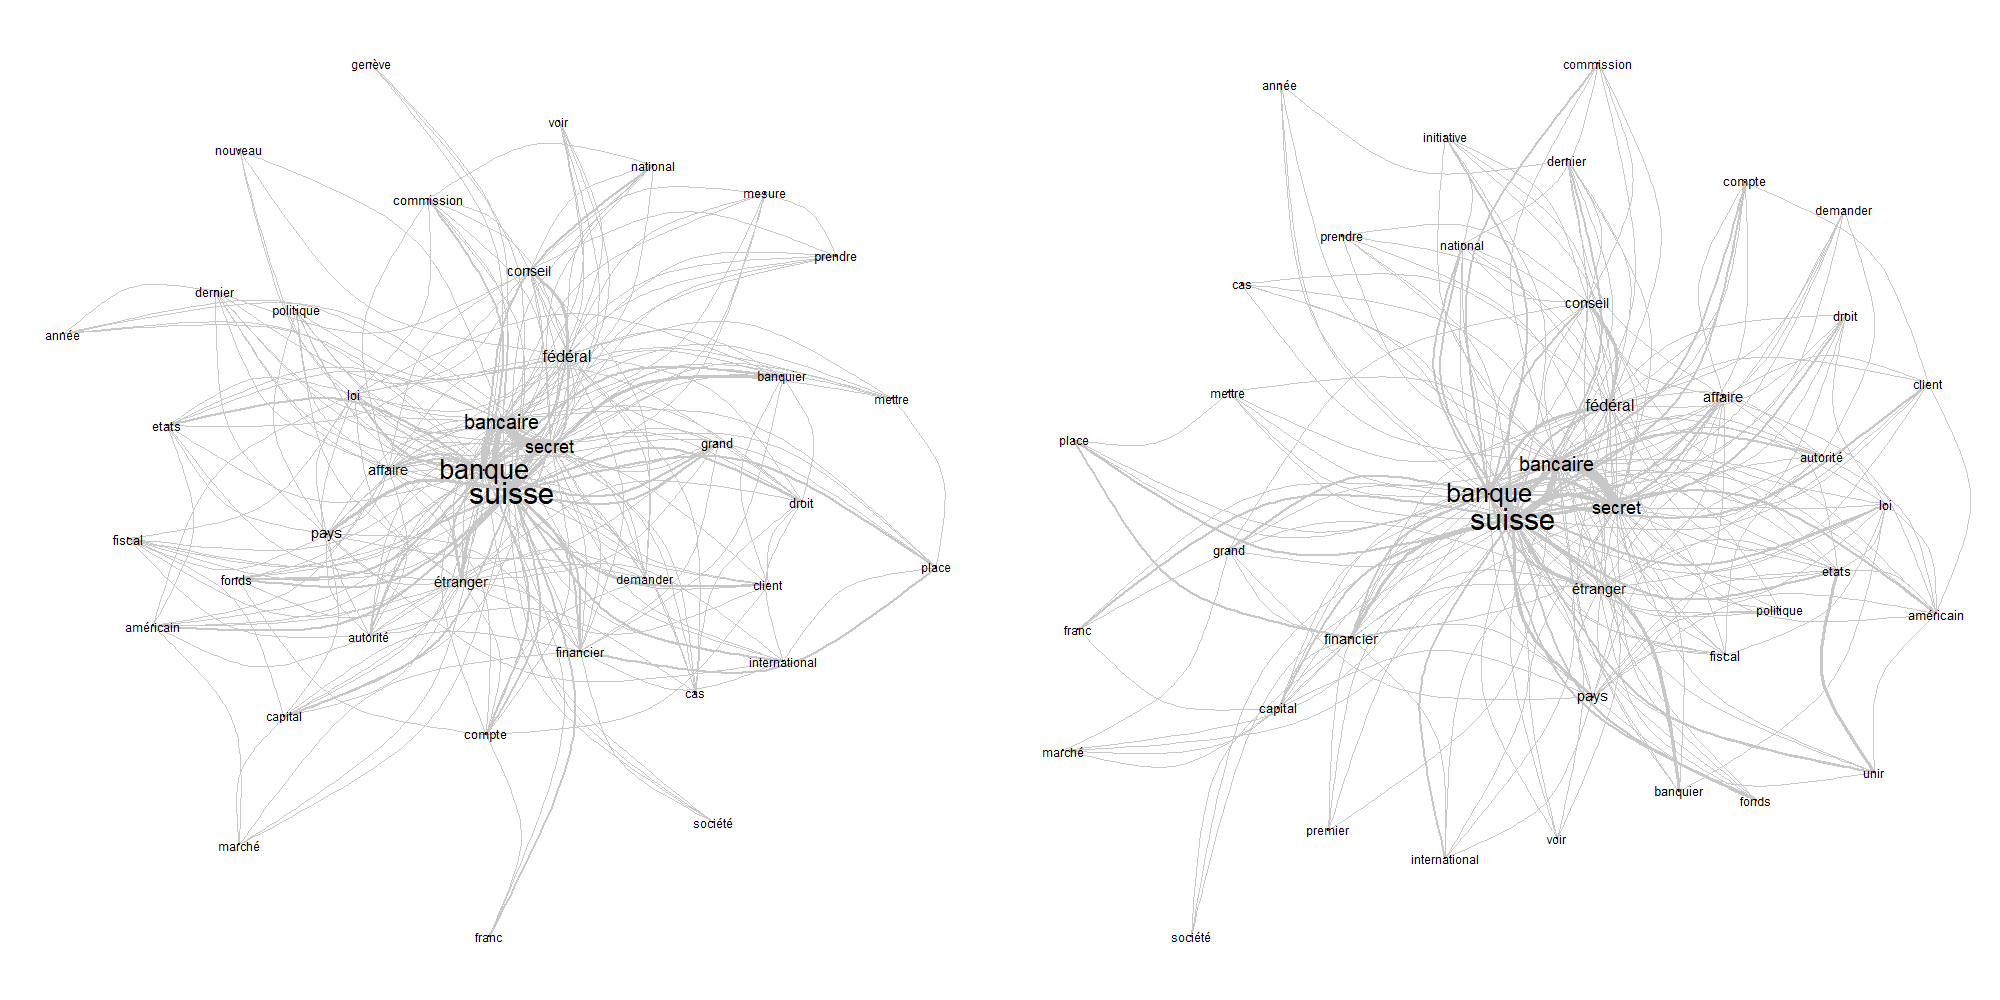
\includegraphics[width=0.9\textwidth,height=\textheight]{similitude.png}
\caption{Graphes de similitudes du \emph{JDG} (gauche) et de la
\emph{GDL} (droite)}
\end{figure}

En regardant le résultat on voit que les mots qui apparaissent souvent
avec ``secret bancaire'' dans les textes de la \emph{GDL} et du
\emph{JDG} sont différents. Pour la \emph{GDL} on voit des mots tel que
``affaire'' qui apparaissent et qu'on ne voit pas dans le résultat avec
le \emph{JDG}.

Afin de rendre les visuels utilisables, nous affichons ici seulement 40
mots (autres que préposition et déterminants). Afin de ne pas surcharger
l'image, seuls les termes qui apparaissent plus de 50 fois ensemble sont
montrés reliés dans le graphe.

En suite, toujours dans un esprit de comparaison des journaux, nous
produisons deux dendrogrammes sur les journaux.

\begin{figure}
\centering
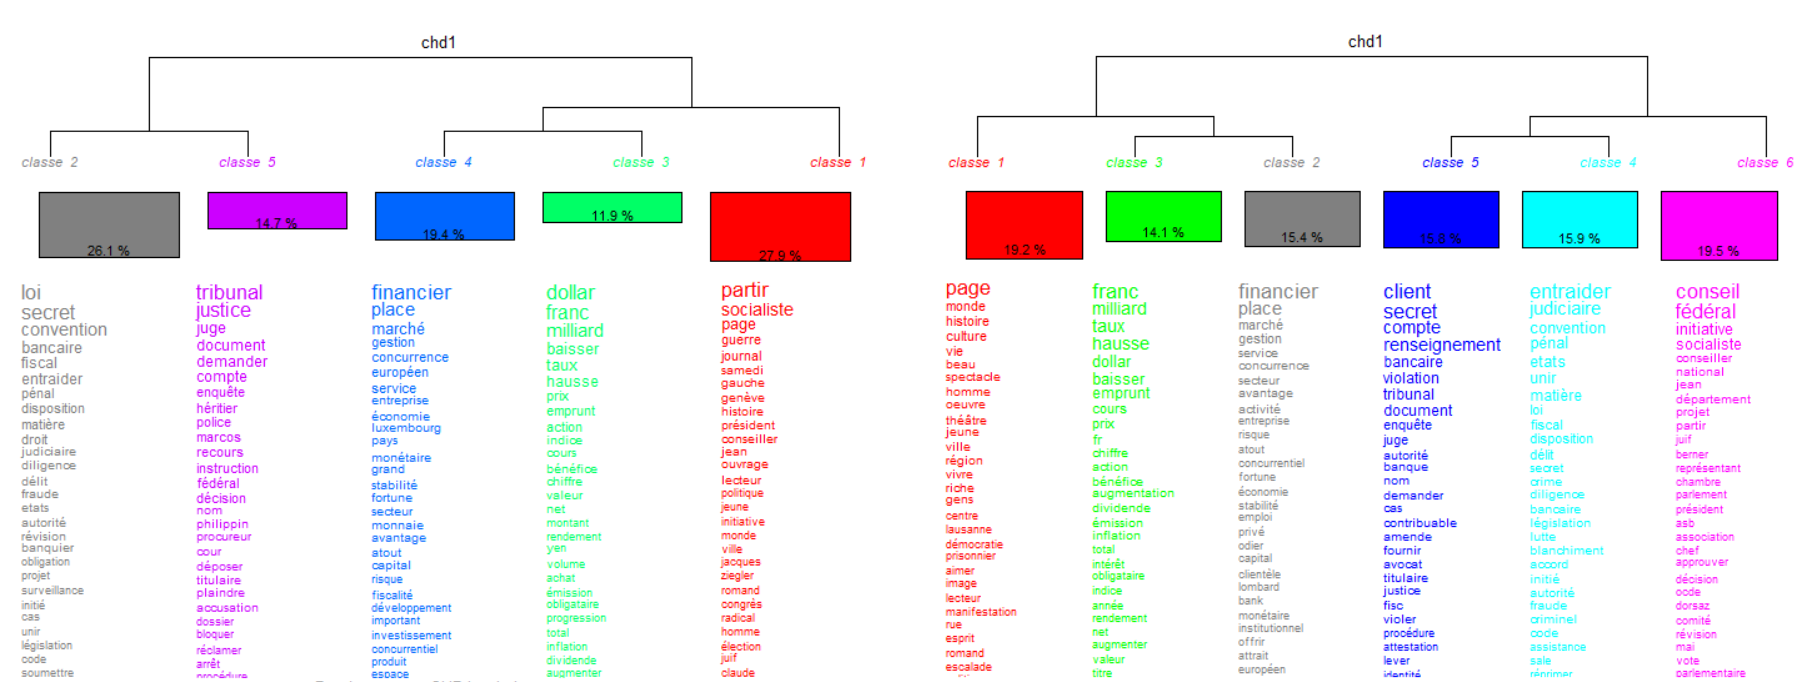
\includegraphics{dendrogram.png}
\caption{Dendrogrammes du \emph{JDG} (gauche) et de la \emph{GDL}
(droite)}
\end{figure}

Cela nous permet de comparer le langage utilisé dans les deux journaux,
nous voyons qu'un journal a été organisé en cinq clusters et l'autre en
six, montrant une divergence dans la façon d'aborder le sujet. Les
champs lexicaux sont proches mais cela nous n'apporte encore rien sur le
contexte d'utilisation des mots.

En poussant cette idée plus loin, nous obtenons les graphes AFC.

Cette visualisation nous présente les distances entre des mots dans le
texte, et nous permet de voir qu'entre les deux journaux le vocabulaire
employé est plus variable dans la gazette de Lausanne.

Avec ces informations, nous pouvons déjà observer que le style
d'écriture des articles est différent. Nous observons par exemple que la
\emph{GDL} semble mettre ensemble des articles qui parlent de secret
bancaire avec des articles qui parlent d'affaires judiciaires (avec les
mots ``secret'', ``bancaire'' proche du mot ``judiciaire'').

\hypertarget{critique-et-difficultuxe9es}{%
\subsubsection{Critique et
difficultées}\label{critique-et-difficultuxe9es}}

Notre analyse est particulièrement perturbée par les problèmes de l'OCR
de basse qualité. Car, les termes que nous tentons d'isoler sont plutôt
long et une erreur de reconnaissance est bien plus probable.

Un autre problème est que le format de reconnaissance des articles est
assez limité. Il a fallu que nous allions chercher le nom des auteurs
manuellement, cependant nous avons observé que mettre le nom de l'auteur
sur un article de journal ne devient courant qu'à partir des années 60,
limitant nos capacité d'analyse avant cette période.

Nous avons réussi à contourner ce problème en utilisant une liste de
noms de journalistes ayant travaillé pour le \emph{JDG}. Cependant nous
n'avons pas trouvé une telle liste pour la \emph{GDL}.

\begin{figure}
\centering
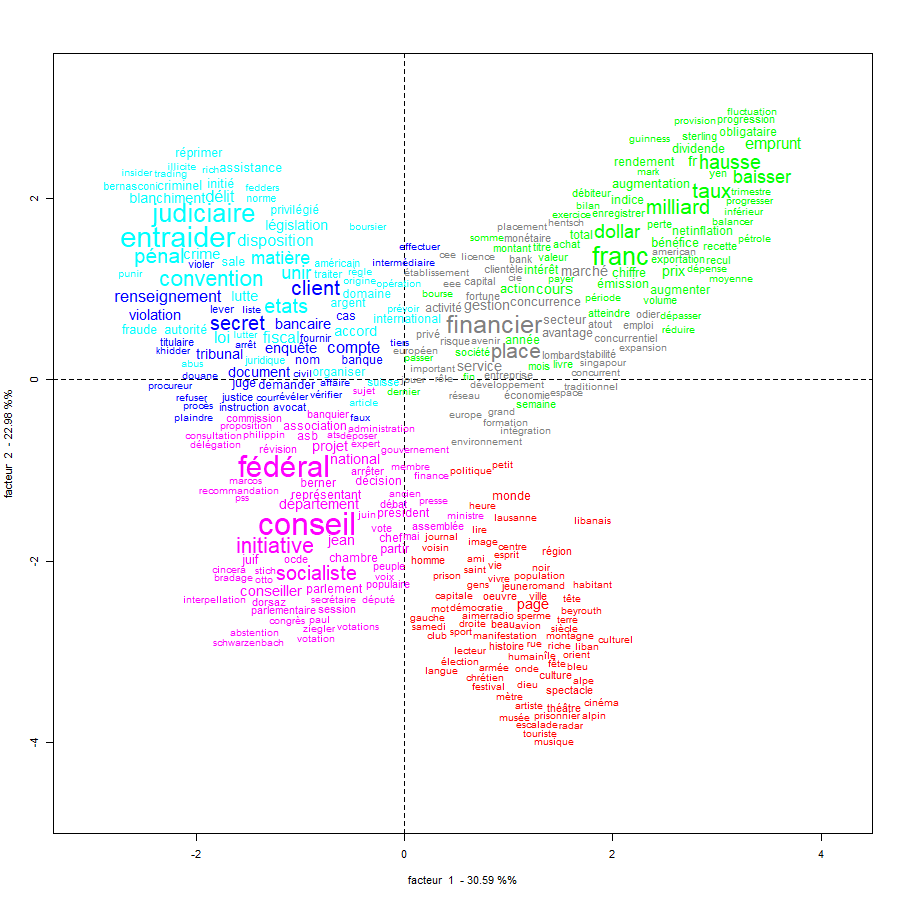
\includegraphics[width=0.8\textwidth,height=\textheight]{AFC2DL_GDL.png}
\caption{AFC de la Gazette de Lausanne}
\end{figure}

\begin{figure}
\centering
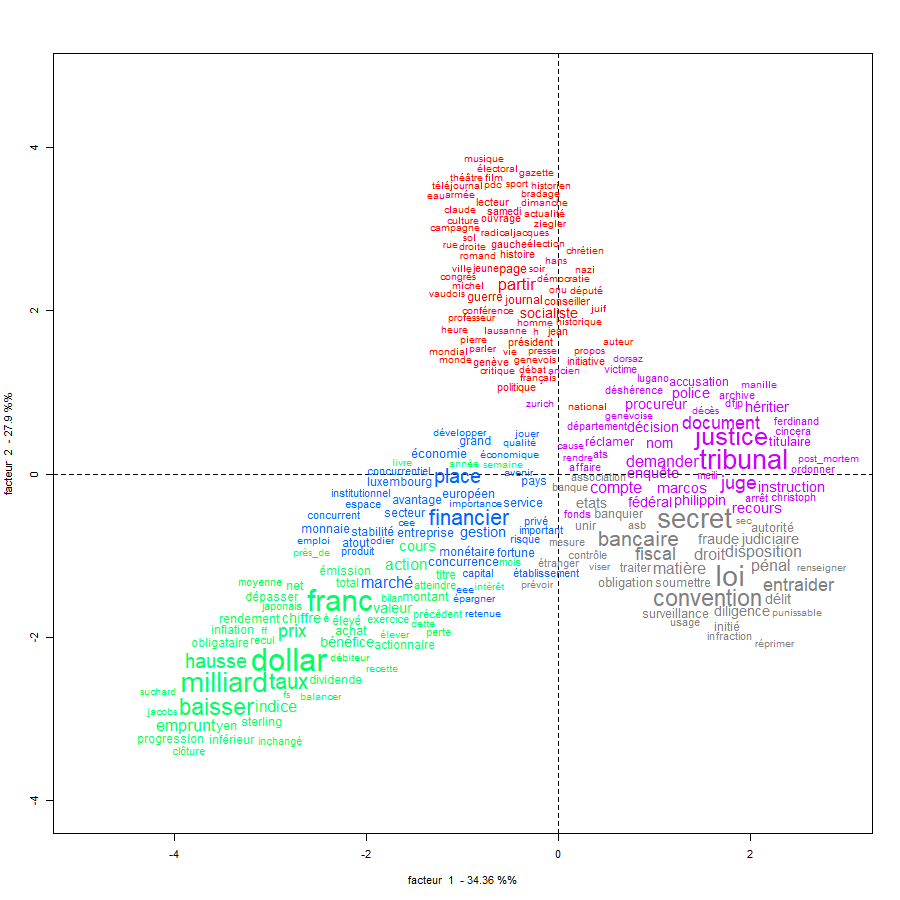
\includegraphics[width=0.8\textwidth,height=\textheight]{AFC2DL_JDG.png}
\caption{AFC du journal de Genève}
\end{figure}
